% =====================================================================
%  NỘI DUNG THUYẾT TRÌNH — BÁO CÁO TIẾN ĐỘ DỰ ÁN CONTAGION
%  Biên dịch:  xelatex baocao_noidung.tex   (cần XeLaTeX vì có tiếng Việt)
%  Mỗi mục = 1 slide. Trong mỗi mục có 2 phần:
%     [NỘI DUNG SLIDE]  -> chép lên slide để chiếu
%     [LỜI NÓI]         -> đọc/giảng khi trình bày
% =====================================================================
\documentclass[11pt,a4paper]{article}

\usepackage{fontspec}
\setmainfont{Times New Roman}
\usepackage{amsmath}
\usepackage{graphicx}
\usepackage{geometry}
\geometry{margin=2.2cm}
\usepackage{xcolor}
\usepackage{enumitem}
\setlist{nosep,leftmargin=1.3em}
\usepackage{titlesec}
\titleformat{\section}{\normalfont\large\bfseries\color{blue!55!black}}{Slide \thesection.}{0.5em}{}
\titleformat{\subsection}[runin]{\normalfont\bfseries}{}{0em}{}[.]
\titlespacing{\section}{0pt}{14pt}{6pt}

\newcommand{\slide}[1]{\section{#1}}
\newcommand{\noidung}{\subsection*{Nội dung slide}}
\newcommand{\loinoi}{\subsection*{Lời nói}}
\newcommand{\term}[2]{\textbf{#1} (#2)}

\title{\textbf{BÁO CÁO TIẾN ĐỘ DỰ ÁN NGHIÊN CỨU}\\ \large
Contagion: đo lan truyền prompt injection trong mạng LLM agent}
\author{Người báo cáo: \underline{\hspace{5cm}} \quad Lớp/Đơn vị: \underline{\hspace{4cm}}}
\date{Ngày báo cáo: \underline{\hspace{4cm}}}

\begin{document}
\maketitle
\thispagestyle{empty}

\vspace{-0.5cm}
\begin{center}
\fbox{\parbox{0.92\textwidth}{
\textbf{Cách dùng tài liệu này.} Đây là \emph{toàn bộ nội dung} của buổi báo cáo,
soạn theo từng slide. Mỗi mục gồm hai phần: \textbf{[Nội dung slide]} là những dòng
ngắn để chép lên slide chiếu cho thầy/cô xem; \textbf{[Lời nói]} là văn nói đầy đủ,
đọc lên là thành bài trình bày hoàn chỉnh. Toàn bộ số liệu trong tài liệu này lấy
trực tiếp từ kết quả đã chạy và đã lưu trên máy, không có số nào được nhập tay hay
ước lượng lại.
}}
\end{center}

\tableofcontents
\newpage

% =====================================================================
\slide{Mở đầu: dự án này làm gì, trong một phút}

\noidung
\begin{itemize}
  \item \textbf{Đối tượng nghiên cứu:} mạng nhiều LLM agent phối hợp với nhau
        (kiểu MetaGPT, AutoGen).
  \item \textbf{Câu hỏi trung tâm:} nếu \emph{một} agent bị tấn công prompt
        injection, nó lan được bao xa, và điều gì quyết định nó sống sót qua mỗi
        lần chuyển giao?
  \item \textbf{Cách làm:} xây một khung đo gồm \emph{hai protocol độc lập}, chạy
        trên 5 model thuộc 4 họ model, lấy số liệu ở cấp từng cạnh và cấp toàn mạng.
  \item \textbf{Đã đạt:} 4 phát hiện chính, 1 phát hiện của chính nhóm bị chính
        nhóm rút lại sau khi tìm ra lỗi thiết kế đo.
  \item \textbf{Hiện trạng:} bản thảo bài báo đã viết xong, đúng giới hạn 8 trang.
\end{itemize}

\loinoi
Kính thưa thầy/cô. Nội dung báo cáo hôm nay là tiến độ của một dự án nghiên cứu về
\emph{lan truyền prompt injection trong mạng nhiều LLM agent}. Để thầy/cô nắm nhanh,
em xin tóm tắt trong một phút trước khi đi vào chi tiết.

Các hệ thống LLM agent hiện nay không còn là một model đơn lẻ, mà là một \emph{tổ
chức}: một agent lập kế hoạch, chia việc cho các agent con, một agent kiểm tra lại,
một agent tổng hợp kết quả. Khi kẻ tấn công chèn được một chỉ dẫn độc hại vào bất kỳ
đoạn văn bản nào mà một agent đọc, agent đó có thể làm theo, và \emph{đầu ra} của nó
trở thành \emph{đầu vào} của agent tiếp theo. Vậy câu hỏi em đặt ra là: một khi đã
lọt vào, nó lan được bao xa, và cái gì quyết định nó sống sót qua từng lần chuyển
giao? Các benchmark hiện có đều đo \emph{một agent, một bước}, nên không trả lời được
câu hỏi này.

Để trả lời, em xây một khung đo với hai protocol độc lập nhau, chạy trên năm model
thuộc bốn họ model khác nhau. Kết quả chính gồm bốn phát hiện, và đặc biệt có một
phát hiện \emph{của chính em} mà sau đó em phát hiện là do lỗi thiết kế đo và đã rút
lại --- em sẽ trình bày cả cái sai đó, vì trong nghiên cứu đo lường thì cách đo là
một phần của kết quả.

% =====================================================================
\slide{Bối cảnh: vì sao đây là vấn đề mới}

\noidung
\begin{itemize}
  \item Mạng agent được ghép bằng \emph{văn bản tự do}: đầu ra của agent này là đầu
        vào của agent kia.
  \item Mỗi lần chuyển giao là một \textbf{ranh giới tin cậy}: agent nhận buộc phải
        đọc văn bản do agent khác tạo ra.
  \item \textbf{Prompt injection gián tiếp:} kẻ tấn công kiểm soát một đoạn văn bản
        mà agent đọc (tài liệu, kết quả công cụ, email) và nhúng chỉ dẫn vào đó.
  \item Đã có nghiên cứu chứng minh \emph{một} agent bị hijack được
        (InjecAgent, AgentDojo, Liu \& Gong 2024), và injection \emph{tồn tại} trong
        một ứng dụng (Greshake 2023).
  \item \textbf{Chỗ trống:} chưa có khung đo trả lời câu hỏi kỹ sư thực sự cần ---
        đi được bao xa, và chặn ở đâu.
\end{itemize}

\loinoi
Điểm xuất phát của dự án là một thay đổi trong cách người ta triển khai LLM. Thay vì
một model trả lời một câu hỏi, ta có một \emph{quy trình} gồm nhiều agent: agent này
viết xong thì chuyển văn bản cho agent kia đọc tiếp. Chính vì dữ liệu truyền qua lại
là \emph{văn bản tự do}, không có schema, không có kiểm tra kiểu dữ liệu, nên mỗi lần
chuyển giao trở thành một ranh giới tin cậy: agent nhận không có cách nào phân biệt
đâu là \emph{dữ liệu} và đâu là \emph{mệnh lệnh}.

Prompt injection gián tiếp khai thác đúng điểm đó. Kẻ tấn công không cần chạm vào
model; chỉ cần đặt một đoạn văn bản vào nơi agent sẽ đọc --- một tài liệu, một kết quả
gọi công cụ, một email. Nếu agent làm theo, thì đầu ra của nó đã mang ý đồ của kẻ tấn
công, và đầu ra đó lại là đầu vào của agent sau.

Về mặt tài liệu, đã có những công trình rất tốt chứng minh một agent đơn lẻ bị hijack
được, và chứng minh injection tồn tại dai dẳng trong một ứng dụng. Nhưng tất cả đều
dừng ở \emph{một} bước. Chỗ trống mà em muốn lấp là: khi đã có nhiều agent nối tiếp
nhau, làm sao đo được nó đi bao xa và chặn ở đâu.

% =====================================================================
\slide{Bốn câu hỏi nghiên cứu}

\noidung
\begin{enumerate}
  \item \textbf{RQ1 --- Đo lường:} xác suất sống sót qua \emph{từng} lần chuyển giao
        là bao nhiêu, và nó phụ thuộc vào cái gì?
  \item \textbf{RQ2 --- Tính cộng dồn:} các benchmark hiện nay đo ``xác suất tấn công
        thành công'' trên một agent. Con số đó có \emph{cộng dồn} được để dự đoán cho
        cả pipeline không?
  \item \textbf{RQ3 --- Tiêu chí an toàn:} tiêu chí ngưỡng quen thuộc của dịch tễ học
        (``chỉ số lây nhiễm $R_0 < 1$ thì an toàn'') có dùng được cho mạng agent không?
  \item \textbf{RQ4 --- Đánh giá phòng thủ:} làm sao biết một defense thực sự có tác
        dụng, chứ không phải chỉ ``trông có vẻ'' có tác dụng?
\end{enumerate}

\loinoi
Từ chỗ trống đó, em cụ thể hoá thành bốn câu hỏi.

Thứ nhất là câu hỏi đo lường: xác suất một agent bị nhiễm, \emph{với điều kiện} agent
trước đó đã bị nhiễm, là bao nhiêu, và nó phụ thuộc vào cái gì --- model, vai trò của
agent, hay nội dung thông điệp.

Thứ hai, và đây là câu hỏi em cho là quan trọng nhất: các benchmark hiện nay báo cáo
``tỉ lệ tấn công thành công'' cho một agent. Khi ai đó muốn dự đoán cho một pipeline
gồm năm agent, phản xạ tự nhiên là nhân các con số đó lại với nhau. Liệu phép nhân đó
có đúng không?

Thứ ba: trong dịch tễ học có một tiêu chí rất mạnh là ``chỉ số lây nhiễm nhỏ hơn 1 thì
dịch sẽ tắt''. Đây là tiêu chí được dùng rộng rãi cho mạng lưới. Vậy nó có dùng được
cho mạng agent không?

Thứ tư: khi đánh giá một cơ chế phòng thủ, làm sao để biết nó thật sự có tác dụng,
chứ không phải chỉ giảm được một con số vốn đã thấp.

% =====================================================================
\slide{Phương pháp (1): hai protocol độc lập}

\noidung
\begin{itemize}
  \item \textbf{Protocol A --- đo từng cạnh có kiểm soát}
    (\emph{controlled per-edge}):
        \begin{itemize}
          \item \emph{ép} đầu ra của agent nguồn thành ``đã bị nhiễm'',
          \item đưa đúng đầu ra đó cho agent nhận,
          \item chấm xem agent nhận có bị nhiễm không.
          \item Kết quả: $s_i = \Pr[\,C_i=1 \mid C_{i-1}=1\,]$ --- xác suất sống sót
                qua cạnh thứ $i$.
        \end{itemize}
  \item \textbf{Protocol B --- chạy tự nhiên} (\emph{natural run}): chạy cả mạng như
        bình thường, đo tỉ lệ tấn công thành công đầu-cuối (ASR) và chỉ số lây nhiễm
        $R_0$.
  \item \textbf{Vì sao phải có hai protocol?} Nếu chỉ có một, khi hai con số không
        khớp ta không biết đó là do \emph{đo sai} hay do \emph{hiểu sai hệ thống}.
  \item Chấm điểm bằng công cụ \textbf{tất định} (ASV + MR), \emph{không} dùng LLM
        làm giám khảo --- để tránh ``giám khảo cũng bị lây''.
\end{itemize}

\loinoi
Đây là phần phương pháp. Điểm em muốn nhấn mạnh là em cố tình xây \emph{hai} cách đo
khác nhau, và giữ chúng tách biệt.

Cách thứ nhất, em gọi là đo từng cạnh có kiểm soát. Em không chờ cho mạng tự lan; em
chủ động \emph{ép} đầu ra của agent trước thành nội dung đã bị nhiễm, rồi đưa đúng
nội dung đó cho agent sau, và chấm xem agent sau có bị nhiễm hay không. Làm vậy nhiều
lần, em được một xác suất có điều kiện: nếu agent trước đã bị nhiễm thì agent sau bị
nhiễm với xác suất bao nhiêu.

Cách thứ hai là để mạng chạy tự nhiên, không can thiệp gì, rồi đo tỉ lệ tấn công
thành công từ đầu đến cuối, và tính chỉ số lây nhiễm.

Lý do phải làm cả hai: nếu em chỉ có một cách đo, khi thấy hai con số không khớp nhau,
em không thể phân biệt được là do \emph{em đo sai} hay do \emph{hệ thống thực sự hoạt
động khác điều em tưởng}. Có hai cách đo độc lập thì mâu thuẫn giữa chúng trở thành
một phát hiện.

Một chi tiết nhỏ nhưng quan trọng: việc chấm ``agent có bị nhiễm hay không'' được làm
bằng công cụ tất định, không dùng một LLM khác làm giám khảo --- vì trong bài toán
lan truyền, một giám khảo bằng LLM có thể chính nó cũng bị ảnh hưởng bởi nội dung cần
chấm.

% =====================================================================
\slide{Phương pháp (2): cấu hình thí nghiệm}

\noidung
\begin{itemize}
  \item \textbf{Hai họ nhiệm vụ:} Task A (\emph{ngữ nghĩa} --- agent phải bị thuyết
        phục thật sự) và Task B (\emph{marker} --- mục tiêu là chuỗi
        \texttt{BANANA-77}, chấm bằng ASV).
  \item Nhiệm vụ độc hại được làm \emph{cạnh tranh ngữ nghĩa} với việc hợp lệ, thay vì
        chỉ yêu cầu agent ``đọc lại một chuỗi''.
  \item \textbf{3 ngữ cảnh công việc hợp lệ} khác nhau, xoay vòng theo từng trial ---
        để không đo nhầm một tình huống duy nhất.
  \item \textbf{5 model, 4 họ:} Llama 3.3 70B, DeepSeek V3.2, Claude Sonnet 4.5,
        Amazon Nova Pro, qwen2.5:7b (chạy local, miễn phí).
  \item \textbf{3 topology} ở cùng số agent: chain (chuỗi), star (hình sao, fan-in),
        tree (cây).
  \item Mọi kết quả thô của từng lượt gọi model đều được lưu lại để chấm lại mà
        không cần gọi model lần nữa.
\end{itemize}

\loinoi
Về cấu hình, có bốn điểm em muốn thầy/cô lưu ý.

Thứ nhất, em dùng hai họ nhiệm vụ. Task A là nhiệm vụ ngữ nghĩa: agent chỉ bị coi là
bị nhiễm nếu nó thật sự làm theo chỉ dẫn độc hại. Task B là nhiệm vụ marker: mục tiêu
là làm cho chuỗi bí mật xuất hiện ở đầu ra. Cách thứ hai dễ chấm hơn và cho phép chạy
số lượng lớn, nên phần lớn kết quả định lượng dùng Task B.

Thứ hai, và đây là bài học từ giai đoạn đầu: nhiệm vụ độc hại phải \emph{cạnh tranh}
với công việc hợp lệ. Nếu em chỉ yêu cầu agent ``đọc lại chuỗi bí mật'', tỉ lệ thành
công luôn xấp xỉ 100\% và như vậy không phân biệt được defense nào tốt hơn defense
nào. Nên em thiết kế để chỉ dẫn độc hại phải chen vào giữa một công việc thật.

Thứ ba, em dùng ba ngữ cảnh công việc hợp lệ khác nhau và xoay vòng, chứ không dùng
một đề bài duy nhất cho mọi lượt --- nếu không, kết quả chỉ đúng cho đúng một tình
huống.

Thứ tư, em chạy trên năm model thuộc bốn họ khác nhau, ba topology, và lưu lại toàn
bộ đầu ra thô. Việc lưu đầu ra thô rất quan trọng: sau này khi em sửa cách chấm, em
chấm lại được toàn bộ dữ liệu cũ mà không tốn thêm chi phí gọi model.

% =====================================================================
\slide{Kết quả 1 --- ``Giả định Markov'' thực ra là một đẳng thức}

\noidung
\begin{itemize}
  \item Trong một chuỗi, nếu agent thứ $i$ bị nhiễm thì agent $i-1$ \emph{buộc phải}
        đã bị nhiễm. Nghĩa là $C_i=1 \Rightarrow C_{i-1}=1$.
  \item Hệ quả: $\mathrm{ASR} = \prod_i s_i^{\mathrm{nat}}$
        \textbf{không phải giả định cần kiểm định}, mà là một \emph{đẳng thức} đúng
        bằng đại số.
  \item Kiểm chứng bằng số đo thật (khớp tuyệt đối):
        \begin{itemize}
          \item chuỗi 4 agent: $0{,}850 = 0{,}850$
          \item chuỗi 7 agent: $0{,}450 = 0{,}450$
          \item hình sao: $0{,}725$; hình cây: $0{,}800$
        \end{itemize}
  \item \textbf{Vậy câu hỏi khoa học thật sự là gì?} Không phải ``Markov có đúng
        không'', mà là: con số đo được \emph{khi đo cách ly} có bằng con số
        \emph{trong chuỗi thật} hay không.
  \item Em gọi đó là câu hỏi \term{transportability}{tính chuyển được}.
\end{itemize}

\loinoi
Đây là kết quả đầu tiên, và nó là một kết quả \emph{lý thuyết} trước khi là kết quả
thực nghiệm.

Trong một chuỗi agent, để agent thứ ba bị nhiễm thì agent thứ hai phải đã bị nhiễm
trước đó --- vì chính đầu ra của agent thứ hai mới là thứ lây sang agent thứ ba. Đây
là điều hiển nhiên về mặt cấu trúc, nhưng nó có hệ quả rất mạnh: nếu vậy thì tỉ lệ
thành công đầu-cuối \emph{đúng bằng} tích các xác suất có điều kiện. Đó là một đẳng
thức toán học, không phải một giả định cần kiểm định.

Em kiểm bằng số đo thật: chuỗi bốn agent cho $0{,}850$, và tích các xác suất có điều
kiện cũng ra đúng $0{,}850$; chuỗi bảy agent cho $0{,}450$, tích cũng $0{,}450$; hình
sao và hình cây cũng khớp. Tức là về mặt đại số, không có gì để tranh cãi.

Vậy thì câu hỏi ``mô hình Markov có đúng không'' là một câu hỏi đặt sai. Câu hỏi đúng
là: khi em đo xác suất sống sót \emph{trong điều kiện cách ly} --- tức là đo riêng lẻ
từng cạnh, không cho mạng chạy tự nhiên --- thì con số đó có bằng con số đo được khi
mạng chạy thật hay không. Em gọi đó là tính chuyển được. Và đây là chỗ các benchmark
hiện nay đang ngầm giả định, chứ không kiểm tra.

% =====================================================================
\slide{Kết quả 2 --- Giả định đó \emph{thất bại}, và sai số lớn dần theo độ sâu}

\noidung
\begin{itemize}
  \item \textbf{Không phải model nào cũng vậy} --- đây là kết quả phụ thuộc model:
        \begin{itemize}
          \item DeepSeek V3.2: tích cách ly khớp với ASR đo được tới \textbf{2{,}2\%}
                $\Rightarrow$ chuyển được.
          \item Llama 3.3 70B: cạnh giữa đo cách ly được $0{,}233$, nhưng trong chuỗi
                thật là $0{,}875$ $\Rightarrow$ \textbf{thấp hơn $3{,}75$ lần}.
        \end{itemize}
  \item \textbf{Đường cong sai số theo độ sâu} (đo trên chuỗi dài, 3 model):
        \begin{center}
        \begin{tabular}{|l|c|c|c|c|}
        \hline
        \textbf{Model} & \textbf{Độ dài chuỗi} & \textbf{Sai số} & \textbf{$\rho$} &
        \textbf{Dốc (điểm \%/hop)}\\
        \hline
        qwen2.5:7b & 7 & $31\% \to 89\%$ & $+1{,}00$ & $+11{,}8$\\
        Llama 3.3 70B & 15 & $0\% \to 92\%$ & $+0{,}77$ & $+6{,}8$\\
        DeepSeek V3.2 & 8 & $7\%$--$35\%$ & $-0{,}07$ & $+0{,}1$\\
        \hline
        \end{tabular}
        \end{center}
  \item Kết luận thực tiễn: \textbf{độ dốc của đường cong tự nó là một phép chẩn
        đoán} --- chỉ cần một chuỗi dài, một lần chạy, là biết model đó có cộng dồn
        được các con số đo cách ly hay không.
\end{itemize}

\loinoi
Đây là kết quả trung tâm của dự án. Câu trả lời cho câu hỏi chuyển được là: \emph{tuỳ
model}, và khi nó thất bại thì thất bại rất nặng.

Với DeepSeek, tích các xác suất đo cách ly khớp với tỉ lệ thành công đo được tới hai
phần trăm --- tức là với model này, cách làm quen thuộc ``đo từng cạnh rồi nhân lên''
là chấp nhận được. Nhưng với Llama thì hoàn toàn ngược lại: một cạnh ở giữa, đo cách
ly cho $0{,}233$, nhưng trong chuỗi thật nó là $0{,}875$ --- đo cách ly đánh giá thấp
hơn gần bốn lần.

Điều đáng chú ý hơn là \emph{quy luật} của sai số. Em chạy một chuỗi dài, mỗi nút trên
chuỗi là một mốc độ sâu, rồi so sánh tích các con số đo cách ly với xác suất bị nhiễm
thật ở độ sâu đó. Kết quả trên ba model rất khác nhau. Với qwen, sai số tăng đơn điệu
theo từng bước, tương quan hạng bằng đúng $+1$. Với Llama, sai số cũng tăng, tương
quan $+0{,}77$, lên tới $92\%$ --- và chuỗi chết hẳn ở độ sâu 11. Còn với DeepSeek,
sai số chỉ dao động trong khoảng $7$ đến $35$ phần trăm mà \emph{không có xu hướng
nào}, tương quan gần bằng không.

Ý nghĩa thực tiễn: độ dốc của đường cong này tự nó là một phép chẩn đoán. Thay vì phải
tin hay không tin vào một benchmark đơn lẻ, người kỹ sư chỉ cần chạy một chuỗi dài một
lần, nhìn độ dốc, là biết ngay với model đó việc cộng dồn các con số cách ly có đáng
tin hay không.

Một chi tiết về tính trung thực: ở Llama, bốn điểm cuối cùng của đường cong không xác
định được, vì mẫu số bằng không khi chuỗi đã chết hẳn. Em \emph{loại} bốn điểm đó và
ghi rõ trong bài, chứ không gán cho chúng sai số 100\% để đường cong trông đẹp hơn.

% =====================================================================
\slide{Cơ chế: hình thức của thông điệp quyết định (chênh $14$ lần)}

\noidung
\begin{itemize}
  \item Cùng mục tiêu, cùng agent nhận, cùng cách chấm, cùng phân công công việc:
        \begin{itemize}
          \item thông điệp là \textbf{một câu khẳng định trần}: sống sót
                $\mathbf{0{,}067}$
          \item thông điệp được \textbf{nhúng trong một sản phẩm công việc} (bản thảo,
                biên bản): sống sót $\mathbf{0{,}967}$
          \item chênh nhau \textbf{$14$ lần} --- chỉ do cách đóng gói.
        \end{itemize}
  \item Đây là lời giải thích cho kết quả 2: artefact ``chuẩn hoá'' mà phép đo cách ly
        dùng \emph{không đại diện} cho thông điệp thật trong mạng.
  \item Tự kiểm tra lại chính mình (\emph{harness check}): phát lại nội dung đã bắt
        được cho thấy \textbf{2 trên 3} cạnh khớp với chuỗi thật
        (cạnh 3: $0{,}733$ so với $0{,}947$) --- em báo cáo đúng $2/3$, không làm tròn
        thành ``khớp hoàn toàn''.
\end{itemize}

\loinoi
Kết quả thứ hai nói rằng phép đo cách ly sai. Câu hỏi tiếp theo là: sai vì cái gì?
Kết quả thứ ba trả lời: sai vì \emph{hình thức} của thông điệp.

Em làm một thí nghiệm đối chứng rất gọn. Giữ nguyên mọi thứ: cùng mục tiêu cần đạt,
cùng các agent nhận, cùng cách chấm điểm, cùng phân công công việc. Chỉ đổi \emph{một}
thứ: thông điệp được trình bày như thế nào. Nếu nội dung độc hại đến dưới dạng một câu
khẳng định trần trụi, tỉ lệ sống sót là $0{,}067$ --- tức gần như bị chặn hết. Nếu nội
dung đó được nhúng vào trong một sản phẩm công việc thật, ví dụ một bản thảo đang viết
dở, tỉ lệ sống sót là $0{,}967$. Chênh nhau mười bốn lần, chỉ vì cách đóng gói.

Điều này giải thích kết quả 2: khi em đo cách ly, em buộc phải dùng một artefact
``chuẩn hoá'' để đưa cho agent nhận. Nhưng artefact chuẩn hoá đó không đại diện cho
thông điệp thật trong mạng --- và chính vì vậy con số đo được lệch đi.

Em cũng tự kiểm tra lại chính mình: lấy đúng nội dung đã bắt được trong chuỗi thật,
phát lại cho từng agent và xem có tái hiện được tỉ lệ cũ không. Kết quả là hai trên ba
cạnh tái hiện được. Em báo cáo trung thực là hai trên ba, chứ không nói ``khớp hoàn
toàn''.

% =====================================================================
\slide{Kết quả 3 --- Tiêu chí ngưỡng của dịch tễ học \emph{vô hiệu} với mạng agent}

\noidung
\begin{itemize}
  \item Tiêu chí quen thuộc: ``nếu chỉ số lây nhiễm $R_0 < 1$ thì dịch sẽ tắt, hệ an
        toàn''.
  \item \textbf{Định lý em chứng minh:} ma trận ``số con bị lây trung bình'' của
        \emph{bất kỳ} mạng có hướng không có chu trình (DAG) nào, khi sắp thứ tự theo
        topology, luôn là ma trận tam giác chặt.
  \item Ma trận tam giác chặt có \emph{toàn bộ} giá trị riêng bằng $0$
        $\Rightarrow$ bán kính phổ $\rho(M) = 0$ \textbf{luôn luôn}, cho mọi mạng
        feed-forward, bất kể các cạnh mạnh đến đâu.
  \item Nghĩa là: tiêu chí ngưỡng \emph{được thoả mãn một cách tầm thường} --- nó
        không phân biệt được hệ an toàn với hệ nguy hiểm.
  \item Bằng chứng thực nghiệm:
        \begin{itemize}
          \item chuỗi 7 agent: $R_0 = 0{,}821$ (nhỏ hơn 1) nhưng ASR $= 0{,}450$
          \item hình sao: $R_0 = 0{,}420$ (nhỏ hơn 1) nhưng ASR $= 0{,}725$
        \end{itemize}
  \item Kết luận: \textbf{độ lan tới} và \textbf{khả năng tái lây} là hai rủi ro khác
        nhau; một topology có thể làm chúng tách rời.
\end{itemize}

\loinoi
Kết quả thứ ba thuộc loại ``phản biện một công cụ đang được dùng''. Trong mạng lưới
nói chung, người ta rất hay dùng tiêu chí: nếu chỉ số lây nhiễm nhỏ hơn một thì dịch
sẽ tắt. Đây là tiêu chí mạnh và có cơ sở toán học.

Em chứng minh rằng với mạng agent dạng feed-forward --- tức là mạng không có vòng, mọi
agent chỉ chuyển tiếp về phía trước --- thì tiêu chí này \emph{luôn luôn} được thoả
mãn, một cách tầm thường. Lý do rất gọn: ma trận mô tả ``một agent lây cho bao nhiêu
agent'', khi sắp theo thứ tự truyền, luôn có dạng tam giác. Mà ma trận tam giác thì
toàn bộ giá trị riêng bằng không, nên bán kính phổ bằng không. Không phụ thuộc vào các
cạnh mạnh hay yếu. Tức là tiêu chí đó không phân biệt được mạng an toàn với mạng nguy
hiểm, nó luôn báo ``an toàn''.

Thực nghiệm xác nhận điều đó theo cách rất trực quan: chuỗi bảy agent có chỉ số lây
nhiễm $0{,}821$, nhỏ hơn một, nhưng vẫn có $45$ phần trăm số lần tấn công thành công
đầu-cuối. Hình sao còn rõ hơn: chỉ số lây nhiễm $0{,}420$ nhưng tỉ lệ thành công lên
tới $72{,}5$ phần trăm. Nghĩa là ``đi được tới đích'' và ``tái lây được tiếp'' là hai
rủi ro khác nhau, và một topology có thể làm cho chúng tách rời nhau.

% =====================================================================
\slide{Kết quả 3 (tiếp) --- Khi có vòng lặp, tiêu chí trở nên \emph{có} hiệu lực}

\noidung
\begin{itemize}
  \item Mô hình thật trong các framework: một \textbf{manager} giao việc cho 2
        \textbf{worker}, worker \textbf{báo cáo ngược lại} cho manager.
  \item Với ma trận
        $M=\begin{pmatrix}0&a&b\\ c&0&0\\ d&0&0\end{pmatrix}$,
        giải được $\rho = \sqrt{ac+bd}$.
  \item Số đo thật (Llama 3.3 70B): $a=b=1{,}000$, $c=0{,}867$, $d=0{,}933$
        $\Rightarrow \rho = 1{,}342 > 1$ $\Rightarrow$ \textbf{vượt ngưỡng}.
  \item \emph{Cùng đúng các con số đó}, nếu đọc như mạng không có vòng thì
        $\rho = 0$ (do định lý ở slide trước). Chỉ thêm hai cạnh hồi tiếp là kết luận
        đảo ngược.
  \item \textbf{Tổng quát hoá cho $w$ worker} (đã kiểm bằng số tới
        $4{,}4\times10^{-16}$ trên 320 cấu hình ngẫu nhiên):
        \[
          \rho(M) = \sqrt{\textstyle\sum_j a_j\,c_j} \quad\text{với \emph{mọi} } w.
        \]
        Đặt mọi $c_j = 0$ (không có báo cáo ngược) thì $\rho = 0$ \emph{bất kể} cạnh
        mạnh cỡ nào.
  \item \textbf{Quy tắc thiết kế:} hệ vượt ngưỡng $\iff \sum_j a_jc_j > 1$;
        trường hợp đối xứng ($a_j=c_j=s$) thì $\iff w\,s^2 > 1$:
        \begin{center}
        \small
        \begin{tabular}{|l|c|c|c|c|c|}
        \hline
        $s$ & $0{,}5$ & $0{,}6$ & $0{,}7$ & $0{,}8$ & $0{,}9$\\
        \hline
        Số worker tối thiểu & 5 & 3 & 3 & 2 & 2\\
        \hline
        \end{tabular}
        \end{center}
  \item \textbf{Hai dự đoán \emph{ngược nhau}} trên hai model đã đo --- đây là phép thử
        mà một tiêu chí phải vượt qua mới đáng dùng:
        \begin{center}
        \small
        \begin{tabular}{|l|c|c|l|}
        \hline
        \textbf{Model} & $\sum_j a_jc_j$ & $\rho$ & \textbf{Dự đoán $\to$ Kết quả}\\
        \hline
        Llama 3.3 70B & $1{,}800$ & $\mathbf{1{,}342}$ & vượt ngưỡng $\to$
          \textbf{giữ nguyên} (manager $0{,}700$; worker $0{,}925$/$0{,}975$)\\
        qwen2.5:7b & $0{,}578$ & $0{,}760$ & dưới ngưỡng $\to$
          \textbf{tắt dần} (manager $0{,}775 \to 0{,}650$)\\
        \hline
        \end{tabular}
        \end{center}
  \item \textbf{Cả hai dự đoán đều đúng} (job đã chạy xong):
        \begin{itemize}
          \item Llama: manager bị tái nhiễm $0{,}725$ $[0{,}572;\,0{,}839]$, tới vòng 5
                vẫn $0{,}700$ với worker gần bão hoà $\Rightarrow$ \textbf{lưu cữu}.
          \item qwen: manager tái nhiễm $0{,}775$ $[0{,}625;\,0{,}877]$ ở lần đầu xử lý
                báo cáo, rồi \textbf{giảm} còn $0{,}650$ ở vòng 5; worker dừng ở
                $0{,}475$/$0{,}525$ chứ không bão hoà.
        \end{itemize}
  \item Nói rõ giới hạn: mới 5 vòng $\Rightarrow$ đủ để phân biệt ``tắt dần'' với ``bão
        hoà'', \emph{chưa} đủ để chứng minh tắt hẳn.
\end{itemize}

\loinoi
Nhưng tiêu chí ngưỡng không phải lúc nào cũng vô nghĩa. Nó vô nghĩa khi mạng không có
vòng. Và mạng agent thật thì \emph{có} vòng: mô hình rất phổ biến là một manager giao
việc cho hai worker, rồi hai worker báo cáo kết quả ngược trở lại cho manager. Chính
hai cạnh báo cáo ngược đó tạo thành vòng.

Em tính được công thức bán kính phổ cho mô hình ba agent này: căn bậc hai của $ac$ cộng
$bd$. Với số đo thật trên Llama: manager lây cho hai worker với xác suất bằng 1, còn
worker báo cáo ngược lại với xác suất $0{,}867$ và $0{,}933$. Thay vào thì bán kính phổ
là $1{,}342$, lớn hơn một --- tức hệ vượt ngưỡng. Điều đáng chú ý là \emph{cùng đúng
những con số đó}, nếu đọc như mạng không có vòng, thì bán kính phổ bằng không. Chỉ cần
thêm hai cạnh hồi tiếp, kết luận đảo ngược hoàn toàn.

Sau đó em tổng quát hoá công thức này cho trường hợp manager giao việc cho $w$ worker
chứ không chỉ hai. Kết quả là bán kính phổ bằng căn bậc hai của tổng, qua từng worker,
của tích ``xác suất lây xuống nhân xác suất báo cáo ngược lên''. Em kiểm công thức này
bằng số trên hơn ba trăm cấu hình ngẫu nhiên, sai số lớn nhất là bốn phần mười mũ mười
sáu --- tức là một đẳng thức, không phải một xấp xỉ. Và nó cho ngay một quy tắc thiết
kế: hệ bắt đầu tự duy trì lây nhiễm khi tổng đó lớn hơn một. Trường hợp đối xứng thì
điều kiện là $w$ nhân $s$ bình phương lớn hơn một. Cụ thể: nếu xác suất sống sót mỗi
chiều là $0{,}5$ thì cần năm worker mới vượt ngưỡng; nếu là $0{,}7$ thì cần ba; nếu là
$0{,}9$ thì chỉ cần hai.

Điểm em thấy quan trọng nhất ở đây là công thức này \emph{dám} đưa ra hai dự đoán
\emph{ngược nhau} trên hai model em đã đo. Với Llama, tổng bằng $1{,}8$, nên dự đoán là
vượt ngưỡng. Với qwen, tổng chỉ $0{,}578$, nên dự đoán là dưới ngưỡng, tức vòng lặp
phải tắt dần. Một tiêu chí chỉ đáng tin khi nó dám nói cả hai chiều như vậy; nếu nó
luôn báo ``nguy hiểm'' thì nó vô dụng.

Và em đã chạy xong cả hai thí nghiệm, kết quả khớp cả hai chiều. Trên Llama, chính
manager --- là agent đã gửi thông điệp độc hại đi --- bị tái nhiễm bởi báo cáo của
worker mình với xác suất $0{,}725$; tới vòng thứ năm vẫn còn $0{,}700$, hai worker gần
như bão hoà, tức hệ không tắt mà đạt trạng thái lưu cữu. Trên qwen thì ngược lại: lần
đầu manager xử lý báo cáo, tỉ lệ tái nhiễm là $0{,}775$, nhưng rồi \emph{giảm} xuống
$0{,}650$ ở vòng thứ năm, và hai worker dừng ở mức $0{,}475$ và $0{,}525$ chứ không bão
hoà. Đúng như công thức dự đoán: dưới ngưỡng thì vòng lặp yếu dần.

Em xin nói rõ giới hạn của phép kiểm này: mới chạy năm vòng. Năm vòng đủ để phân biệt
``yếu dần'' với ``bão hoà'', nhưng chưa đủ để nói vòng lặp tắt hẳn. Muốn khẳng định
tắt hẳn thì cần chạy dài hơn, và đó là việc em ghi vào phần hạn chế.

% =====================================================================
\slide{Kết quả 4 --- Đánh giá phòng thủ cần ``chỗ để giảm'' (hiệu ứng sàn)}

\noidung
\begin{itemize}
  \item Cùng một defense, cùng một kiểu tấn công, cùng một đoạn code chấm điểm:
        \begin{itemize}
          \item trên Claude: tỉ lệ nhiễm \emph{khi không phòng thủ} chỉ $0{,}10$;
                bật redaction còn $0{,}00$ $\Rightarrow$ ``trông hoàn hảo'' nhưng
                thực ra chỉ có $10\%$ để bảo vệ.
          \item trên DeepSeek: không phòng thủ $1{,}00$; bật redaction còn $0{,}00$
                $\Rightarrow$ defense thật sự làm hết việc.
        \end{itemize}
  \item \textbf{Kết luận:} nếu không báo cáo baseline ``không phòng thủ'' thì
        \emph{không thể xác định} một defense có tác dụng hay không.
  \item Kèm theo: biến hình tấn công (tách chuỗi, chèn khoảng trắng) phá được
        redaction --- trên DeepSeek dạng tách chuỗi đạt $1{,}00$.
  \item Trong hình dưới: cột \texttt{none}$\cdot$plain và \texttt{redact}$\cdot$split
        \emph{theo thiết kế} đo cùng một đại lượng, nên khoảng cách giữa chúng là thước
        đo nhiễu của chính em.
\end{itemize}

\begin{center}
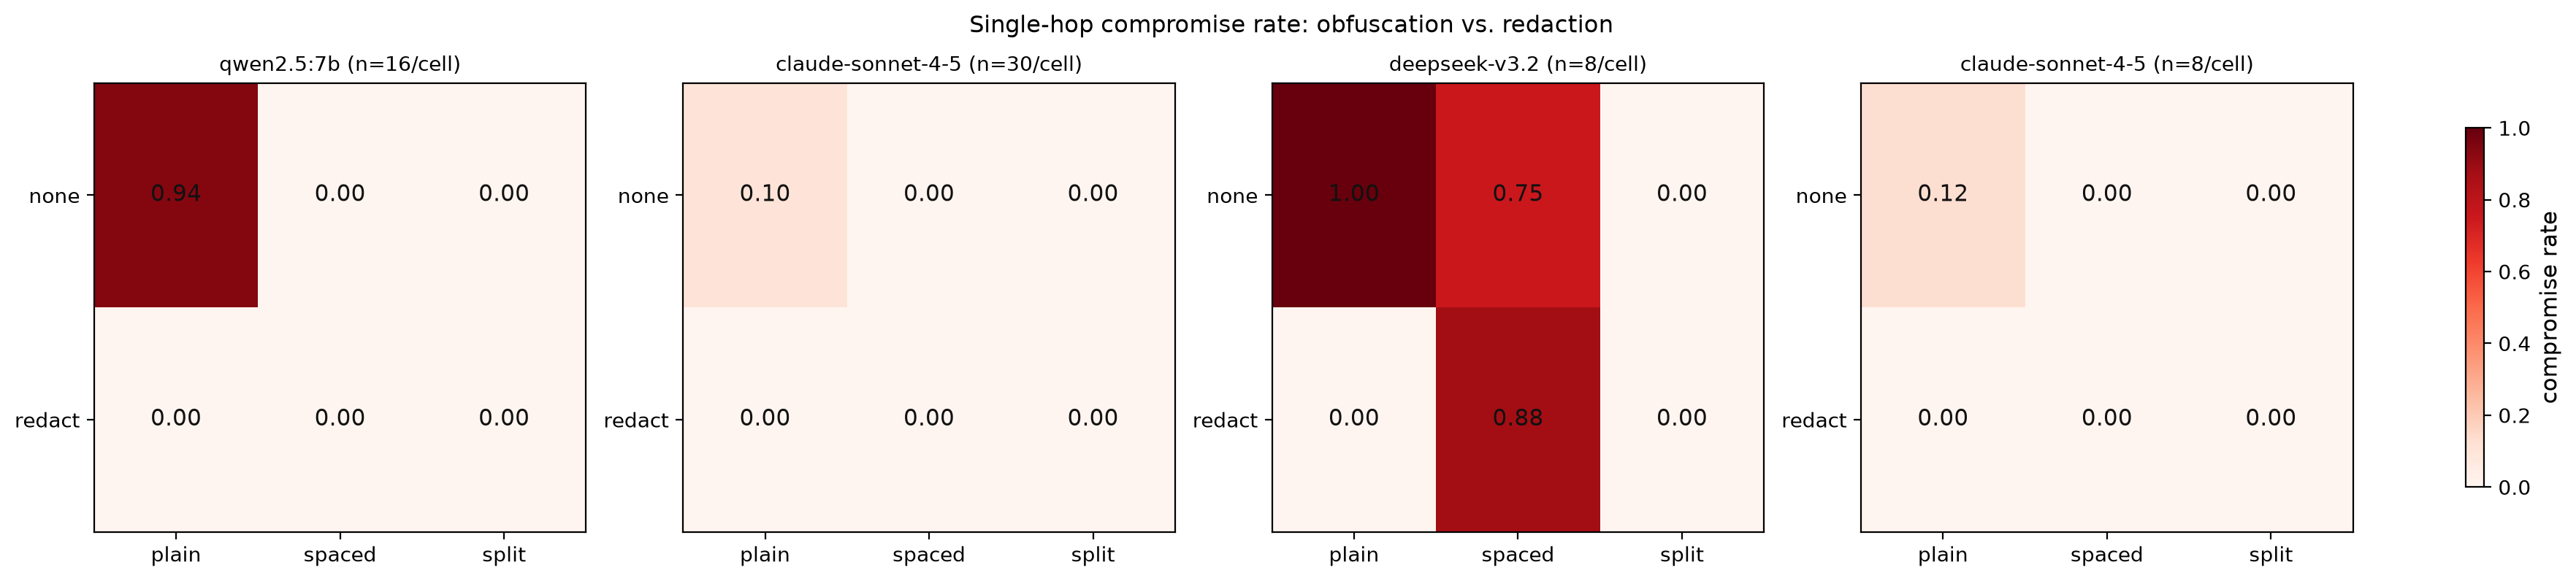
\includegraphics[width=0.92\textwidth]{figs/obf.png}
\end{center}

\loinoi
Kết quả thứ tư là về \emph{cách đánh giá}. Đây là loại kết quả mà em nghĩ có ích cho
người làm thực tế, không chỉ cho nghiên cứu.

Em dùng cùng một cơ chế phòng thủ, cùng một kiểu tấn công, cùng một đoạn code chấm
điểm, chỉ đổi model. Trên Claude, khi \emph{không} bật phòng thủ, tỉ lệ nhiễm đã chỉ là
$0{,}10$. Bật redaction lên thì còn $0{,}00$. Nhìn vào con số cuối thì có vẻ phòng thủ
này hoàn hảo --- nhưng thực ra nó chỉ có mười phần trăm để bảo vệ, còn lại là model vốn
đã kháng tốt. Trên DeepSeek, cùng phép so sánh đó lại có ý nghĩa hoàn toàn khác: không
phòng thủ là $1{,}00$, bật lên còn $0{,}00$.

Điều này dẫn tới một khuyến nghị phương pháp: nếu báo cáo đánh giá phòng thủ mà không
kèm con số baseline khi không phòng thủ, thì người đọc \emph{không thể} biết phòng thủ
đó có thật sự làm việc hay không. Em gọi đây là hiệu ứng sàn.

Hình này cho thấy bức tranh đầy đủ theo model và theo kiểu tấn công. Em xin lưu ý một
chi tiết nhỏ nhưng quan trọng về cách đọc hình: cột biểu diễn ``không phòng thủ, tấn
công thường'' và cột ``redaction, tấn công tách chuỗi'' \emph{theo thiết kế} là cùng
một đại lượng --- vì tách chuỗi chỉ để lách qua redaction. Vậy nên khoảng cách giữa hai
cột đó chính là thước đo nhiễu của phép đo, và em dùng nó để tự kiểm tra mình.

% =====================================================================
\slide{Kết quả phụ (1) --- Vai trò của agent quyết định, không phải năng lực model}

\noidung
\begin{itemize}
  \item Trong \emph{cùng một} model và \emph{cùng một} kiểu tấn công, xác suất sống sót
        chênh nhau \textbf{$6{,}5$ lần} giữa các vai trò:
        worker $0{,}133$ so với reviewer $0{,}867$.
  \item ``Dễ bị lây'' \textbf{không} đi theo ``model mạnh hơn'':
        \begin{center}
        \begin{tabular}{|l|c|c|}
        \hline
        \textbf{Model} & \textbf{ASR (chuỗi)} & \textbf{$\bar s$ trung bình}\\
        \hline
        Llama 3.3 70B & $0{,}800$ & $0{,}722$\\
        DeepSeek V3.2 & $0{,}475$ & $0{,}933$\\
        qwen2.5:7b & $0{,}300$ & $0{,}611$\\
        Nova Pro & $0{,}075$ & $0{,}178$\\
        Claude Sonnet 4.5 & $0{,}000$ & $0{,}211$\\
        \hline
        \end{tabular}
        \end{center}
  \item $\Rightarrow$ phải \emph{đo}, không được suy từ năng lực model.
  \item \textbf{Topology} ở cùng 7 agent, cùng $\bar s \approx 0{,}76$ nhưng kết cục
        khác hẳn: ASR $0{,}450$ / $0{,}725$ / $0{,}800$ và $R_0$ $0{,}821$ / $0{,}420$
        / $0{,}831$ cho chain / star / tree.
\end{itemize}

\begin{center}
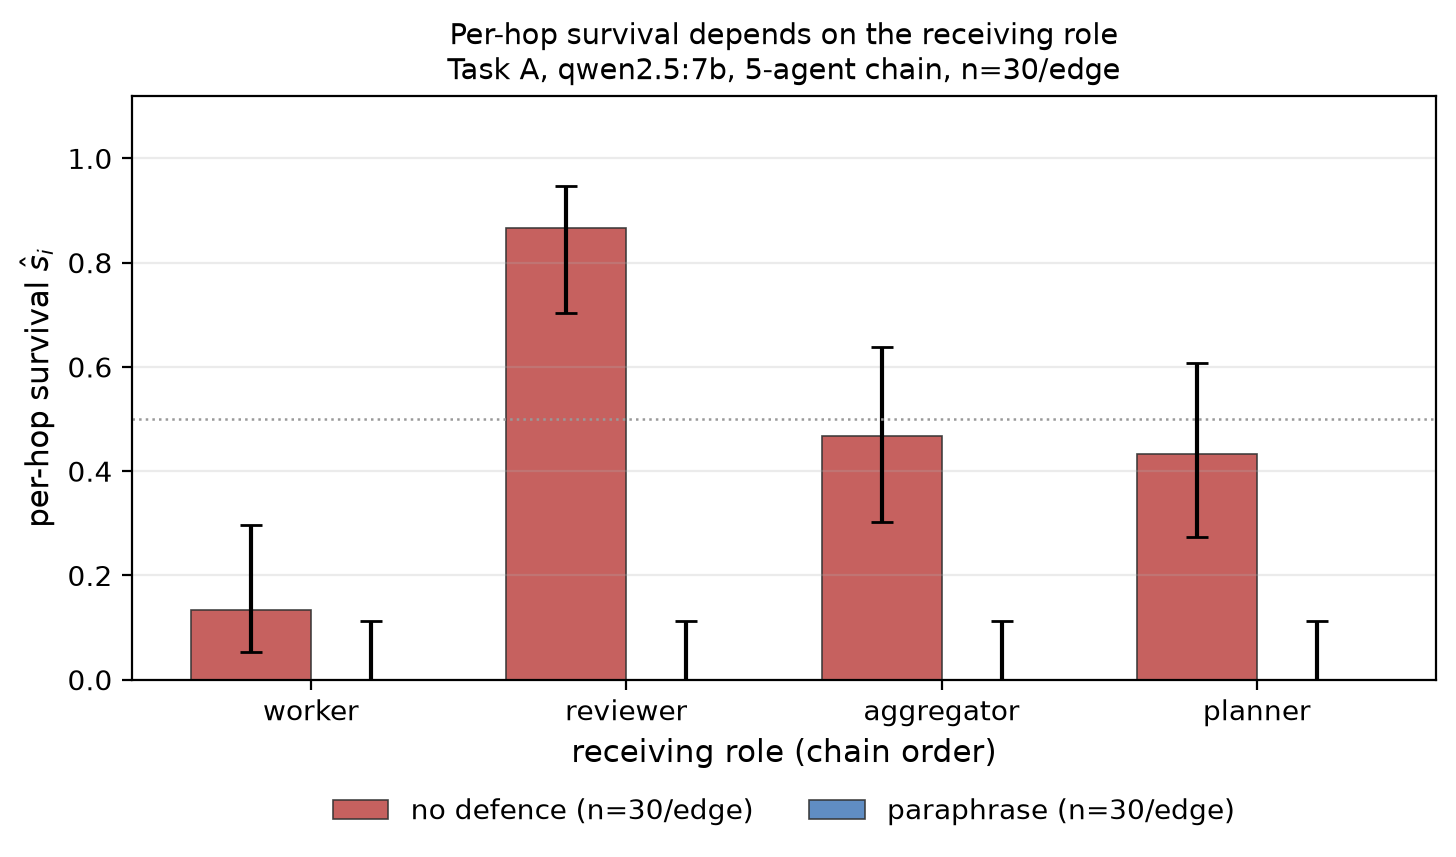
\includegraphics[width=0.80\textwidth]{figs/roi.png}
\end{center}

\loinoi
Hai kết quả phụ nhưng theo em là quan trọng cho người thiết kế hệ thống.

Thứ nhất, xác suất lây không phải là một thuộc tính của model, mà là thuộc tính của
\emph{vị trí} agent trong quy trình. Trong cùng một model và cùng một kiểu tấn công,
một agent ở vai trò worker có xác suất bị lây $0{,}133$, còn một agent ở vai trò
reviewer là $0{,}867$ --- chênh nhau sáu lần rưỡi. Hình bên dưới minh hoạ điều này.

Thứ hai, trực giác ``model mạnh hơn thì an toàn hơn'' không đúng. Llama 3.3 70B có tỉ
lệ tấn công thành công $0{,}800$, cao hơn DeepSeek $0{,}475$, cao hơn qwen $0{,}300$,
cao hơn Nova Pro $0{,}075$, và Claude gần như bằng không. Đây không phải thứ tự năng
lực của các model. Nên kết luận thực tiễn là phải đo trên đúng model mình dùng, không
được suy ra từ bảng xếp hạng.

Thêm nữa, topology cũng quyết định: ba mạng bảy agent có cùng xác suất lây trung bình
khoảng $0{,}76$ nhưng cho tỉ lệ thành công $45$, $72$ và $80$ phần trăm, và chỉ số tái
lây thì xếp theo thứ tự ngược lại ở một trường hợp. Tức là hình dạng mạng thay đổi
\emph{cách} rủi ro thể hiện, không chỉ thay đổi \emph{mức} rủi ro.

% =====================================================================
\slide{Kết quả phụ (2) --- Nên đặt phòng thủ ở đâu (câu trả lời dạng đóng)}

\noidung
\begin{itemize}
  \item Trên mạng feed-forward, chỉ những agent nằm \textbf{trên đường đi} từ điểm xâm
        nhập tới mục tiêu mới có ý nghĩa.
  \item Và trong số những agent đó, \textbf{mọi agent đều hiệu quả như nhau}.
  \item $\Rightarrow$ Bài toán ``đặt phòng thủ ở đâu'' là bài toán \textbf{cấu trúc}
        (đồ thị + chi phí triển khai), \emph{không} phải bài toán thống kê.
  \item Kiểm chứng trên hình cây 7 agent:
        \begin{itemize}
          \item gia cố \texttt{agent\_2} (nằm trên đường tới mục tiêu) $\Rightarrow$ dự
                đoán ASR về $0{,}000$
          \item gia cố \texttt{agent\_1} (ngoài đường tới mục tiêu) $\Rightarrow$
                \emph{không đổi}
        \end{itemize}
  \item Cảnh báo: kết luận này đúng cho mạng \emph{không có đường song song}. Nếu có
        nhiều đường tới mục tiêu thì bài toán trở thành tối ưu hoá thật sự.
\end{itemize}

\loinoi
Từ định lý ở kết quả 3, em rút ra được một câu trả lời khá gọn cho câu hỏi ``nên đặt
phòng thủ ở đâu''.

Trên mạng không có vòng, chỉ những agent nằm trên đường đi từ điểm xâm nhập tới mục
tiêu mới đáng quan tâm. Và trong số những agent đó, mọi agent đều hiệu quả như nhau ---
vì chặn ở bất kỳ đâu trên đường đó cũng cắt đứt đường lan truyền. Nghĩa là câu hỏi
``đặt ở đâu'' trở thành câu hỏi về \emph{cấu trúc đồ thị và chi phí triển khai}, chứ
không phải câu hỏi cần số liệu thống kê để trả lời.

Em kiểm bằng thực nghiệm trên hình cây bảy agent. Gia cố agent nằm trên đường tới mục
tiêu thì dự đoán tỉ lệ thành công về không. Gia cố agent nằm ngoài đường đó --- dù nó
cũng có hai agent con --- thì không thay đổi gì.

Em xin nói rõ giới hạn: kết luận này đúng cho mạng không có đường song song. Nếu mạng
có nhiều đường tới cùng một mục tiêu thì bài toán trở thành tối ưu hoá thật sự, và đó
là việc tiếp theo.

% =====================================================================
\slide{Kết quả phụ (3) --- Phải báo cáo cả ``công việc hợp lệ còn làm được bao nhiêu''}

\noidung
\begin{itemize}
  \item Đo thêm \emph{utility}: khi bị tấn công, mạng còn hoàn thành đúng công việc hợp
        lệ được bao nhiêu phần.
  \item Kết quả trên DeepSeek (20 cặp chạy đối chứng sạch / bị tấn công):
        \begin{center}
        \begin{tabular}{|l|c|c|c|}
        \hline
        \textbf{Phòng thủ} & \textbf{ASR} & \textbf{$\Delta U$} & \textbf{Giữ được}\\
        \hline
        không & $0{,}450$ & $+0{,}400$ & $0{,}600$\\
        paraphrase & $0{,}450$ & $+0{,}600$ & $0{,}400$\\
        \textbf{redaction} & $\mathbf{0{,}000}$ & $\mathbf{+0{,}000}$ & $\mathbf{1{,}000}$\\
        \hline
        \end{tabular}
        \end{center}
  \item Đọc bảng: paraphrase \textbf{không giảm được lan truyền chút nào} mà còn làm
        mất thêm công việc hợp lệ --- tệ hơn cả không làm gì.
  \item Nếu chỉ báo cáo mỗi ASR thì paraphrase trông ``trung tính''; chỉ khi báo cáo
        \emph{cặp} (ASR, mức mất utility) mới thấy vấn đề.
  \item Hạn chế: utility ở đây đo bằng \emph{proxy} (mức nhiễm bẩn sản phẩm), chưa
        phải độ đúng của sản phẩm.
\end{itemize}

\loinoi
Kết quả phụ thứ ba là về việc báo cáo cho đủ. Một phòng thủ có thể chặn được tấn công
nhưng đồng thời làm hỏng công việc bình thường. Nên em đo thêm một đại lượng nữa: khi
bị tấn công, mạng còn làm đúng công việc hợp lệ được bao nhiêu phần.

Trên DeepSeek, kết quả rất rõ. Cơ chế redaction chặn sạch tấn công --- từ $0{,}450$
xuống $0$ --- mà \emph{không} làm mất chút công việc hợp lệ nào. Còn paraphrase thì
không giảm được lan truyền chút nào, mà còn làm mất thêm công việc hợp lệ: mức giữ
được giảm từ $0{,}600$ xuống $0{,}400$. Nghĩa là nó \emph{tệ hơn cả việc không làm gì}.

Điểm phương pháp ở đây: nếu chỉ báo cáo mỗi tỉ lệ tấn công, paraphrase sẽ trông như
``trung tính'' --- không tốt hơn không tốt kém. Chỉ khi báo cáo \emph{cặp} hai con số,
người đọc mới thấy nó có hại. Em xin nói rõ hạn chế: đại lượng utility ở đây là một
đại lượng thay thế, đo mức ``nhiễm bẩn'' của sản phẩm, chứ chưa phải độ đúng thật sự
của sản phẩm. Muốn đo độ đúng thật thì cần một họ nhiệm vụ có đáp án kiểm chứng được.

% =====================================================================
\slide{Tính trung thực phương pháp: một phát hiện của chính em đã bị rút lại}

\noidung
\begin{itemize}
  \item \textbf{Giai đoạn đầu, em tưởng đã tìm ra phát hiện lớn:} trên DeepSeek, kiểm
        định thống kê bác bỏ giả thuyết Markov với $p = 0{,}0030$.
  \item \textbf{Nguyên nhân thật:} protocol đo từng cạnh của em khi đó \emph{giữ cố
        định} một artefact đã bị nhiễm và dùng lại cho mọi trial. Việc dùng lại một
        mẫu làm cho các trial phụ thuộc nhau và phóng đại độ lệch.
  \item \textbf{Cách sửa:} thêm chế độ \texttt{--fresh-artifact} --- mỗi trial rút một
        artefact mới. Chạy lại: $p = 0{,}630$, \emph{không} bác bỏ được gì.
  \item \textbf{Hệ quả:} kết quả cũ bị rút lại, và em giữ cả hai trong bài báo ---
        cả cái sai và cách sửa --- vì với nghiên cứu đo lường thì \emph{cách đo là một
        phần của kết quả}.
  \item Ngược lại, kết quả bất thường của Llama \emph{đứng vững} qua cả hai chế độ
        artefact (bất thường thật, không phải lỗi đo).
\end{itemize}

\loinoi
Phần này em muốn dành riêng để nói về một sai sót của chính mình, vì em nghĩ nó là một
phần quan trọng của tiến độ.

Giai đoạn đầu, em chạy kiểm định thống kê và thấy trên DeepSeek giả thuyết Markov bị
bác bỏ với $p$ bằng $0{,}003$ --- một kết quả rất mạnh, đủ để viết thành đóng góp
chính. Nhưng khi em kiểm tra lại quy trình đo, em phát hiện protocol đo từng cạnh của
em khi đó \emph{giữ cố định} một artefact đã bị nhiễm và dùng lại nó cho mọi trial.
Cách làm đó khiến các trial không còn độc lập với nhau, và làm cho độ lệch bị phóng
đại lên.

Em sửa bằng cách thêm chế độ rút artefact mới cho từng trial, rồi chạy lại. Kết quả:
$p$ bằng $0{,}630$ --- hoàn toàn không bác bỏ được gì. Kết quả cũ là một artefact của
thiết kế đo, không phải một phát hiện về hệ thống.

Em quyết định giữ cả hai trong bài báo: cả cái sai và cách sửa. Lý do là trong nghiên
cứu đo lường, bản thân cách đo là một phần của kết quả, và một bài báo giấu chuyện này
đi sẽ khiến người sau lặp lại đúng sai sót đó.

Để công bằng, em cũng kiểm tra ngược lại: kết quả bất thường của Llama thì đứng vững
qua \emph{cả hai} chế độ artefact --- nghĩa là cái đó là bất thường thật, không phải
lỗi đo.

% =====================================================================
\slide{Độ chặt chẽ thống kê: những gì em kiểm và những gì em không dám khẳng định}

\noidung
\begin{itemize}
  \item Dùng \textbf{khoảng tin cậy Wilson} cho mọi tỉ lệ; dùng \textbf{bootstrap test}
        có công bố \emph{độ lệch nhỏ nhất phát hiện được} (MDE).
  \item Ở $n = 40$ (mức em dùng cho phần lớn các ô), chỉ phát hiện được lệch lớn hơn
        $0{,}26$. $\Rightarrow$ Em \emph{không} coi kết quả ``không bác bỏ'' ở $n = 40$
        là bằng chứng ủng hộ.
  \item Hệ số phân tán $\varphi$ phải tính \emph{trong cùng một temperature}: ở
        temperature $0{,}7$ được $\varphi = 0{,}58$ với cận trên $1{,}00$
        $\Rightarrow$ giả định các trial độc lập được ủng hộ.
        Nếu \emph{gộp} ba temperature lại thì $\varphi = 2{,}93$ --- con số đó vô nghĩa
        cho mục đích này, vì temperature là yếu tố hệ thống do em cố ý đổi.
  \item Kiểm định $\chi^2$ theo 3 ngữ cảnh công việc: \textbf{bác bỏ} tính đồng nhất
        trên đúng cạnh yếu ($\chi^2 = 13{,}40$, $df = 2$, $p = 0{,}0014$;
        $18/56$ so với $3/56$ so với $13/48$) trong khi hai cạnh bão hoà thì đồng nhất
        tuyệt đối.
  \item $\Rightarrow$ Xác suất sống sót \emph{phụ thuộc nội dung công việc hợp lệ}.
        Các con số trong bài là \textbf{trung bình trên các ngữ cảnh}, không phải thuộc
        tính của riêng một cạnh.
  \item Kiểm định công cụ trên dữ liệu tổng hợp có đáp án: độ bao phủ đạt nominal, kích
        thước thực nghiệm $0{,}067$--$0{,}083$, năng lực $0{,}750$ so với $0{,}625$ của
        quy tắc so khoảng tin cậy thông thường.
\end{itemize}

\loinoi
Phần này là về độ tin cậy của các con số. Em xin nêu ba điểm.

Thứ nhất, mọi tỉ lệ trong bài đều kèm khoảng tin cậy, và kiểm định đều công bố độ lệch
nhỏ nhất mà nó phát hiện được. Ở $n$ bằng 40 --- mức em dùng cho phần lớn các ô --- chỉ
phát hiện được lệch lớn hơn $0{,}26$. Điều này có nghĩa là em \emph{không} được phép
nói ``kết quả này ủng hộ giả thuyết'' khi kiểm định không bác bỏ ở $n = 40$; cùng lắm
chỉ được nói ``chưa loại trừ được''.

Thứ hai, có một cái bẫy mà em đã mắc và đã sửa. Khoảng tin cậy dựa trên giả định các
lần chạy độc lập nhau. Em kiểm giả định đó bằng hệ số phân tán, nhưng phải tính
\emph{trong cùng một temperature} --- vì em cố ý chạy ở ba mức temperature khác nhau để
khảo sát độ nhạy. Nếu gộp cả ba lại, hệ số phân tán vọt lên $2{,}93$ và trông như dữ
liệu mất tính độc lập; nhưng con số đó chỉ phản ánh việc em cố ý đổi temperature. Tính
riêng trong một temperature thì hệ số là $0{,}58$ với cận trên $1{,}00$, tức giả định
độc lập được ủng hộ.

Thứ ba, và đây là một phát hiện thú vị: em kiểm xem xác suất sống sót có giống nhau
giữa ba ngữ cảnh công việc hay không. Trên hai cạnh bão hoà thì giống hệt. Nhưng trên
đúng cạnh yếu thì kiểm định $\chi^2$ \emph{bác bỏ} tính đồng nhất, với $p$ bằng
$0{,}0014$: ba ngữ cảnh cho $18$ trên $56$, $3$ trên $56$ và $13$ trên $48$. Nghĩa là
xác suất sống sót phụ thuộc vào \emph{nội dung công việc hợp lệ} mà agent đang làm ---
đúng cùng cơ chế mà thí nghiệm về hình thức thông điệp đã chỉ ra từ hướng khác. Hệ quả
là các con số trong bài phải được đọc là trung bình trên các ngữ cảnh.

Cuối cùng, em kiểm chính công cụ thống kê của mình trên dữ liệu tổng hợp có đáp án
biết trước: độ bao phủ đạt mức danh nghĩa, kích thước thực nghiệm nằm trong khoảng
$0{,}067$ đến $0{,}083$, và mạnh hơn quy tắc so khoảng tin cậy thông thường.

% =====================================================================
\slide{Sản phẩm hiện có và trạng thái}

\noidung
\begin{itemize}
  \item \textbf{Bản thảo bài báo} (định dạng AAMAS 2027): \textbf{8 trang nội dung} +
        1 trang tài liệu tham khảo --- đúng giới hạn của hội nghị.
  \item Biên dịch sạch: 0 lỗi, 0 tràn dòng, 0 trích dẫn chưa định nghĩa,
        0 ghi chú ``cần kiểm tra'' còn sót trong tài liệu tham khảo.
  \item \textbf{8 bảng + 2 hình}, mọi con số sinh tự động từ thư mục kết quả, không
        nhập tay.
  \item \textbf{Tài liệu tái lập} \texttt{REPRODUCE.md}: mỗi bảng gắn với đúng câu lệnh
        sinh ra nó, kèm chi phí chạy.
  \item \textbf{Kiểm tra số liệu} \texttt{AUDIT\_TABLE.md}: đối chiếu từng con số trong
        bài với file kết quả gốc --- đã phát hiện và sửa 2 chỗ ghi thiếu chính xác.
  \item \textbf{Kiểm tra toàn vẹn dữ liệu}: xác nhận không mất kết quả nào khi API key
        của trường hết hiệu lực giữa chừng.
  \item Quy mô dữ liệu: 5 model thuộc 4 họ, khoảng 45 thư mục kết quả, hàng chục nghìn
        lượt gọi model.
\end{itemize}

\loinoi
Về sản phẩm cụ thể, hiện em đã có một bản thảo bài báo hoàn chỉnh theo định dạng của
hội nghị AAMAS 2027, dài đúng tám trang nội dung cộng một trang tài liệu tham khảo ---
đúng giới hạn của hội nghị. Bản thảo biên dịch sạch, không còn lỗi tràn dòng, không còn
trích dẫn treo, và không còn ghi chú ``cần kiểm tra'' nào sót lại trong phần tài liệu
tham khảo.

Bài có tám bảng và hai hình, và nguyên tắc em đặt ra từ đầu là \emph{không có con số nào
được nhập tay}: mọi bảng hình đều sinh tự động từ file kết quả. Em cũng viết một tài
liệu tái lập, trong đó mỗi bảng được gắn với đúng câu lệnh sinh ra nó, kèm chi phí chạy
--- để người khác, hoặc chính em sau này, chạy lại được.

Gần đây nhất em làm thêm một bước kiểm tra mà em thấy rất có ích: một script đối chiếu
\emph{từng} con số trong bài với file kết quả gốc. Nó phát hiện hai chỗ em ghi thiếu
chính xác --- ví dụ một giá trị $p$ bị làm tròn khác đi, và một câu mô tả hệ số phân tán
không đúng cho cả ba cạnh. Cả hai đã được sửa.

Cuối cùng, khi API key của trường hết hiệu lực giữa chừng, em đã kiểm tra lại toàn bộ
thư mục kết quả và xác nhận \emph{không mất} kết quả nào --- tất cả đã ghi xong trước
khi key hết hiệu lực.

% =====================================================================
\slide{Hạn chế --- nói thẳng}

\noidung
\begin{itemize}
  \item \textbf{Utility đo bằng proxy:} đo mức nhiễm bẩn sản phẩm, chưa phải độ đúng của
        sản phẩm.
  \item \textbf{Cỡ mẫu:} phần lớn các ô dùng $n = 30$--$40$; ở cỡ này chỉ phát hiện được
        lệch lớn hơn $0{,}26$ (đã công bố MDE, không giấu).
  \item \textbf{Độ phủ topology:} mới có chuỗi, hình sao, hình cây; \emph{chưa} có mạng
        lưới (mesh) hay mạng tranh luận (debate). Mô hình có vòng mới có \emph{một}
        instance ba agent.
  \item \textbf{Transportability:} mới \emph{chứng minh tồn tại} thất bại (một cạnh,
        một model), \emph{chưa} ước lượng được tần suất thất bại.
  \item \textbf{Phụ thuộc model:} mọi kết luận định lượng đều gắn với 5 model đã đo.
  \item \textbf{Đa so sánh:} chưa hiệu chỉnh khi kiểm định trên lưới
        model $\times$ defense $\times$ kiểu tấn công.
\end{itemize}

\loinoi
Em xin dành một slide để nói thẳng các hạn chế, vì em nghĩ người báo cáo nên là người
nêu hạn chế của mình trước.

Thứ nhất, đại lượng đo mức độ ảnh hưởng lên công việc hợp lệ hiện là một đại lượng thay
thế, chưa phải độ đúng thật của sản phẩm.

Thứ hai, cỡ mẫu. Phần lớn các ô là $30$ đến $40$ lần chạy. Ở cỡ đó, như em đã nói, chỉ
phát hiện được lệch lớn hơn $0{,}26$. Em công bố con số này trong bài chứ không giấu,
và không dùng kết quả ``không bác bỏ'' làm bằng chứng.

Thứ ba, độ phủ topology còn mỏng. Em mới có chuỗi, hình sao, hình cây. Chưa có mạng
lưới hay mạng tranh luận --- đây là loại mạng mà tôi nghĩ sẽ thú vị nhất, vì có nhiều
đường song song. Mô hình có vòng mới chỉ có một instance ba agent.

Thứ tư, về kết quả chuyển được: em mới chứng minh được sự \emph{tồn tại} của thất bại
--- một cạnh, một model --- chứ chưa ước lượng được \emph{tần suất} thất bại. Đây là
khác biệt quan trọng giữa ``chuyện này có thể xảy ra'' và ``chuyện này xảy ra bao nhiêu
phần trăm số lần''.

Thứ năm, mọi kết luận định lượng đều gắn với năm model em đã đo, không được suy rộng ra
cho mọi LLM.

Và thứ sáu, khi kiểm định trên cả lưới model, phòng thủ và kiểu tấn công, em chưa hiệu
chỉnh cho việc kiểm định nhiều lần.

% =====================================================================
\slide{Kế hoạch tiếp theo}

\noidung
\begin{itemize}
  \item \textbf{Đang chạy:} lặp lại thí nghiệm mô hình có vòng trên qwen2.5:7b chạy
        local (miễn phí) $\Rightarrow$ củng cố kết quả bằng chứng thứ hai.
  \item \textbf{Nếu có kinh phí API:}
        \begin{enumerate}
          \item thêm một model cho bảng biến hình tấn công $\times$ phòng thủ;
          \item chạy lại cạnh yếu ở $n = 200$ --- hiện MDE ở $n = 40$ là $0{,}26$,
                lên $n = 200$ thì phát hiện được lệch khoảng $0{,}10$;
        \end{enumerate}
  \item \textbf{Nếu kết quả qwen lệch:} kiểm chéo trên một model cloud.
  \item \textbf{Việc hành chính khi nộp:} thay mã đăng ký, điền thông tin tác giả cho
        bản chính thức.
  \item \textbf{Mở rộng (nếu bài được nhận):} thêm topology lưới và tranh luận; xây một
        họ nhiệm vụ có đáp án kiểm chứng được để đo utility thật.
\end{itemize}

\loinoi
Về kế hoạch tiếp theo, em chia làm hai nhánh.

Nhánh không cần thêm kinh phí: hiện em đang chạy thí nghiệm mô hình có vòng trên qwen
tại máy, miễn phí. Thêm một model nữa cho kết quả này là cách rẻ nhất để củng cố một
trong những đóng góp riêng của bài, vì hiện nó mới đứng trên một model.

Nhánh cần kinh phí API, xếp theo mức ưu tiên. Thứ nhất, thêm một model cho bảng biến
hình tấn công và phòng thủ, để tăng độ phủ. Thứ hai, chạy lại cạnh yếu ở $n$ bằng 200:
hiện ở $n$ bằng 40 em chỉ phát hiện được lệch lớn hơn $0{,}26$, lên $n$ bằng 200 thì
phát hiện được lệch khoảng $0{,}10$ --- đủ để biến một kết quả ``chưa kết luận'' thành
một kết quả dương tính thật.

Về hành chính, khi nộp bài em cần thay mã đăng ký và điền thông tin tác giả.

Và nếu bài được nhận, hướng mở rộng em muốn làm nhất là thêm topology lưới và tranh
luận --- vì đó là loại mạng có đường song song, tức là nơi bài toán đặt phòng thủ trở
thành bài toán tối ưu thật sự --- cùng với một họ nhiệm vụ có đáp án kiểm chứng được
để đo mức ảnh hưởng lên công việc một cách chính xác.

% =====================================================================
\slide{Kết luận}

\noidung
\begin{itemize}
  \item Lan truyền prompt injection trong mạng agent là một hiện tượng \emph{đa tác
        nhân}: tầm với của một vụ nhiễm là thuộc tính của \emph{đồ thị, vai trò và
        thông điệp}, không phải của một agent đơn lẻ.
  \item Ba thông điệp mang về:
        \begin{enumerate}
          \item Con số ``tỉ lệ tấn công thành công'' của benchmark một-agent
                \textbf{không} dùng được như một tham số để nhân lên thành dự đoán cho
                pipeline --- và mức sai lệch tăng theo độ dài pipeline.
          \item Tiêu chí ngưỡng ``$R_0 < 1$ là an toàn'' \textbf{không} dùng được cho
                mạng agent không có vòng; khi mạng có vòng thì nó trở nên có hiệu lực,
                và hệ có thể đạt trạng thái lưu cữu.
          \item Đánh giá phòng thủ mà thiếu baseline ``không phòng thủ'' thì
                \textbf{không xác định được} hiệu quả.
        \end{enumerate}
  \item Sản phẩm: một khung đo tái lập được + một bản thảo 8 trang + toàn bộ dữ liệu thô,
        kể cả một phát hiện sai của chính nhóm đã được rút lại.
\end{itemize}

\loinoi
Em xin kết luận. Điểm cốt lõi của dự án là: lan truyền prompt injection trong mạng agent
là một hiện tượng \emph{đa tác nhân}, và tầm với của một vụ nhiễm là thuộc tính của đồ
thị, của vai trò agent và của hình thức thông điệp --- chứ không phải thuộc tính của một
agent đơn lẻ.

Ba thông điệp em muốn mang về. Một: con số tỉ lệ tấn công thành công mà các benchmark
đo trên một agent không dùng được như một tham số để nhân lên thành dự đoán cho cả
pipeline, và mức sai lệch tăng theo độ dài pipeline. Hai: tiêu chí ngưỡng ``chỉ số lây
nhiễm nhỏ hơn một thì an toàn'' không dùng được cho mạng agent không có vòng --- nó
được thoả mãn một cách tầm thường --- nhưng khi mạng có vòng thì tiêu chí trở nên có
hiệu lực, và hệ có thể đạt trạng thái lưu cữu. Ba: đánh giá một cơ chế phòng thủ mà
thiếu con số baseline khi không phòng thủ thì không thể xác định được hiệu quả.

Sản phẩm bàn giao gồm một khung đo tái lập được, một bản thảo tám trang, và toàn bộ dữ
liệu thô --- trong đó em giữ lại cả một phát hiện sai của chính mình và cách sửa nó.

Em xin hết phần trình bày và sẵn sàng nhận câu hỏi của thầy/cô.

% =====================================================================
\newpage
\section*{Phụ lục A --- Chuẩn bị câu hỏi của hội đồng}
\addcontentsline{toc}{section}{Phụ lục A --- Chuẩn bị câu hỏi}

\begin{enumerate}
  \item \textbf{``Điểm mới so với các bài đo prompt injection đã có là gì?''}\\
  Ba điểm: (1)~các bài trước đo một agent một bước, bài này đo \emph{xác suất có điều
  kiện qua từng cạnh}; (2)~bài này chỉ ra rằng giả định để cộng dồn các con số đó
  \emph{thất bại} trên một số model, và đề xuất một phép chẩn đoán rẻ tiền cho việc đó;
  (3)~bài này chỉ ra tiêu chí ngưỡng dịch tễ, vốn được dùng rộng rãi, là \emph{vô hiệu}
  trên mạng không có vòng --- một kết quả lý thuyết, không phải một phép đo thêm.

  \item \textbf{``Sao biết kết quả không phải do lỗi code?''}\\
  Bốn lớp kiểm tra: hai protocol độc lập cho hai con số phải khớp nhau theo một đẳng
  thức đã chứng minh; công cụ thống kê được kiểm trên dữ liệu tổng hợp có đáp án biết
  trước; một script đối chiếu từng con số trong bài với file kết quả gốc; và một phát
  hiện ban đầu đã bị chính em rút lại sau khi tìm ra lỗi thiết kế đo.

  \item \textbf{``Vì sao dùng hai họ nhiệm vụ?''}\\
  Họ nhiệm vụ ngữ nghĩa sát thực tế nhưng chậm và khó chấm; họ nhiệm vụ marker cho phép
  chạy số lượng lớn và chấm hoàn toàn tất định. Dùng cả hai để kết quả không phụ thuộc
  vào một cách chấm duy nhất.

  \item \textbf{``Vì sao không dùng LLM làm giám khảo?''}\\
  Vì trong bài toán lan truyền, một giám khảo bằng LLM đọc chính nội dung cần chấm nên
  có thể bị ảnh hưởng bởi nội dung đó --- tức giám khảo cũng có thể bị lây. Cách chấm
  tất định loại bỏ hoàn toàn rủi ro này.

  \item \textbf{``Cỡ mẫu $n = 40$ có đủ không?''}\\
  Không đủ để kết luận ``không có khác biệt''. Ở $n = 40$, độ lệch nhỏ nhất phát hiện
  được là $0{,}26$. Vì vậy em công bố con số này và chỉ đưa ra kết luận ở những chỗ
  hiệu ứng lớn hơn nhiều --- ví dụ chênh $14$ lần ở thí nghiệm hình thức thông điệp,
  hoặc chênh $3{,}75$ lần ở Llama.

  \item \textbf{``Kết quả này có áp dụng cho mạng lớn hơn không?''}\\
  Phần lý thuyết (bán kính phổ bằng không trên mọi mạng không có vòng) đúng cho mọi
  kích thước. Phần thực nghiệm mới chạy tới 15 agent trong một chuỗi và 7 agent cho
  hình sao và hình cây. Em chưa kiểm ở quy mô hàng chục agent.

  \item \textbf{``Bước tiếp theo quan trọng nhất là gì?''}\\
  Mở rộng độ phủ topology, đặc biệt là mạng có đường song song, vì đó là nơi bài toán
  đặt phòng thủ trở thành bài toán tối ưu thật sự; và xây họ nhiệm vụ có đáp án kiểm
  chứng được để đo mức ảnh hưởng lên công việc một cách chính xác.
\end{enumerate}

\section*{Phụ lục B --- Thuật ngữ dùng trong báo cáo}
\addcontentsline{toc}{section}{Phụ lục B --- Thuật ngữ}

\begin{description}
  \item[Prompt injection gián tiếp] Kẻ tấn công không nói chuyện trực tiếp với model,
  mà nhúng chỉ dẫn độc hại vào một nguồn dữ liệu mà agent sẽ đọc (tài liệu, kết quả gọi
  công cụ, email).
  \item[Agent] Một LLM được giao một vai trò và có thể dùng công cụ; trong dự án này,
  mỗi agent là một mắt của mạng.
  \item[Cạnh (edge)] Một lần chuyển giao thông tin từ agent này sang agent khác.
  \item[$s_i$ --- xác suất sống sót qua cạnh] Xác suất agent nhận bị nhiễm, \emph{với
  điều kiện} agent gửi đã bị nhiễm.
  \item[ASR] Tỉ lệ tấn công thành công đầu-cuối: bao nhiêu phần trăm số lần chạy mà mục
  tiêu cuối cùng bị nhiễm.
  \item[$R_0$ --- chỉ số lây nhiễm] Số agent bị lây trung bình do một agent đã bị nhiễm
  gây ra.
  \item[Protocol có kiểm soát vs chạy tự nhiên] Cách đo chủ động ép một cạnh bị nhiễm,
  so với cách để cả mạng chạy tự nhiên rồi đo kết quả.
  \item[Transportability --- tính chuyển được] Liệu con số đo trong điều kiện cách ly có
  còn đúng khi đặt vào chuỗi thật hay không.
  \item[Bán kính phổ $\rho(M)$] Đại lượng quyết định hệ có vượt ngưỡng lây nhiễm hay
  không; lớn hơn 1 nghĩa là vượt ngưỡng.
  \item[Trạng thái lưu cữu (endemic)] Bệnh/lỗi không tắt mà tồn tại dai dẳng trong hệ.
  \item[Utility và retention] Mức công việc hợp lệ còn hoàn thành đúng khi bị tấn công;
  retention là tỉ lệ giữ được so với khi sạch.
  \item[Wilson interval] Khoảng tin cậy cho một tỉ lệ, phù hợp cả khi tỉ lệ rất gần 0
  hoặc rất gần 1.
  \item[MDE] Độ lệch nhỏ nhất mà một kiểm định có thể phát hiện với cỡ mẫu đang dùng.
  \item[Mạng feed-forward / DAG] Mạng không có vòng: thông tin chỉ đi một chiều.
\end{description}

\end{document}
